%% LyX 2.2.3 created this file.  For more info, see http://www.lyx.org/.
%% Do not edit unless you really know what you are doing.

\documentclass[10pt,twocolumn,american]{article}
\usepackage[sc]{mathpazo}
\usepackage[scaled=0.9]{helvet}
\renewcommand{\ttdefault}{lmtt}
\usepackage[T1]{fontenc}
\usepackage[latin9]{inputenc}
\usepackage[a4paper]{geometry}
\geometry{verbose,lmargin=1.7cm,rmargin=1.7cm}
\usepackage{fancyhdr}
\pagestyle{fancy}
\setcounter{secnumdepth}{0}
\setcounter{tocdepth}{3}
\setlength{\parskip}{\smallskipamount}
\setlength{\parindent}{0pt}
\usepackage{babel}
\usepackage{float}
\usepackage{enumitem}
\usepackage{graphicx}
\usepackage{todonotes}
\usepackage[unicode=true,
 bookmarks=true,bookmarksnumbered=false,bookmarksopen=false,
 breaklinks=false,pdfborder={0 0 0},backref=false,colorlinks=false]
 {hyperref}
\makeatletter

% User specified LaTeX commands.
% Customization file for the titlepage and document
%************************************************************
% Required stuff
%************************************************************
\usepackage{graphicx}
\usepackage{euler}
\usepackage[detect-all]{siunitx}
\usepackage{sectsty}
\usepackage[font={footnotesize }]{caption}
\usepackage{multicol}
\usepackage{prettyref}

\allsectionsfont{\rmfamily}

% Page customization
\usepackage{fancyhdr}
\pagestyle{fancy}

% Color
\usepackage{color}
\definecolor{light-gray}{gray}{0.85}
\definecolor{dark-gray}{gray}{0.75}

\fancyhead{}  % clear all header fields
\fancyhead[LO,RE]{\rule[-2ex]{0pt}{2ex}\fontsize{9}{11} \selectfont \myPhase : \myTitle}
\fancyhead[CO,CE]{\fontsize{9}{11} \selectfont \myIPT}
\fancyfoot{}  % clear all footer fields
\fancyfoot[LO,LE]{\fontsize{8}{11} \selectfont {\sscap{Website}} : \url{https://github.com/fcuzzocrea/MSAS2017}}
\fancyfoot[RO,LE]{\fontsize{5}{11} \selectfont 
\includegraphics[height=0.18cm]{gfx/CC}  This work is licensed under a Creative Commons Attribution-ShareAlike 4.0 International License.}
\fancyheadoffset[LE,RO]{0.2pt}
\renewcommand{\headrulewidth}{0.2pt}
\renewcommand{\footrulewidth}{0.2pt}
\renewcommand{\headrule}{\hbox to\headwidth{%
   \leaders\hrule height \headrulewidth\hfill}}
\renewcommand{\footrule}{\hbox to\headwidth{%
    \leaders\hrule height \headrulewidth\hfill}}
\hypersetup{colorlinks=true, linkcolor=blue ,linktoc=page,citecolor=black}

%************************************************************
% Redefining numbering for sections
%************************************************************
%\renewcommand*\thesection{\arabic{section}}

%************************************************************
% Cross reference set-up
%************************************************************
\newrefformat{tab}{Table\,\ref{#1}}
\newrefformat{fig}{Figure\,\ref{#1}}
\newrefformat{eq}{Eq.\,\textup{(\ref{#1})}}
\newrefformat{sec}{Sec.\,\ref{#1}}
\newrefformat{sub}{Sec.\,\ref{#1}}

%************************************************************
% Fancy stuff
%************************************************************
\newcommand{\titlecap}[1]{\Huge{\textrm{#1}}}
\newcommand{\subtitlecap}[1]{\Large{\textsc{#1}}}
\newcommand{\sscap}[1]{\textbf{#1}}
\newcommand{\strong}[1]{\textbf{#1}}
\setlength{\headheight}{60pt} %%or

%************************************************************
% Helpful stuff to modify here, not in the LyX Document
%************************************************************
\newcommand{\myDate}{\today}
\newcommand{\myGroup}{}
\newcommand{\myUrl}{\url{https://github.com/fcuzzocrea/MSAS2017}}
\newcommand{\myUni}{}

\newcommand{\myPhase}{Modeling and Simulation of Aerospace Systems}
\newcommand{\myProject}{}
\newcommand{\myIPT}{}
\newcommand{\myTitle}{LISA Pathfinder Final Report}
\newcommand{\myAuthorf}{Alfonso Collogrosso}
\newcommand{\myAuthors}{Francescodario Cuzzocrea}
\newcommand{\myAuthort}{Andrea Mastrantuono}
\newcommand{\myEmail}{}

\newcommand{\mail}[1]{\href{mailto:#1}{\texttt{#1}}}

\setlength{\textfloatsep}{\baselineskip}

\makeatother

\begin{document}

\title{ \titlecap{\Large \myPhase} \rule{\linewidth}{0.01mm}  {\myTitle}}
\date{\today}
\author{\textbf{Authors} : {\myAuthorf, \myAuthors, \myAuthort}}

% Put the abstract fullpage
\twocolumn[
\begin{@twocolumnfalse}
	\maketitle
	\rule{\linewidth}{0.5mm}
		\begin{abstract}
			The LISA scientific space mission will detect gravitational waves by measuring the relative displacement of a pairs of free floating test masses set into geodesic motion on-board of three spacecraft. Inside each satellite, the injection of the test masses from the caged configuration into the geodesic trajectory will be performed by the Grabbing Positioning and Relased Mechanism (GPRM). To provide a successful injection, the test masses must be relased with a minimal residual velocity against the adhesion with the holding device.
In the following document we will proceed trough the derivation and the integration of the system of linear ODEs that describes the forementioned grabbing positioning and relase mechanism.

		\end{abstract}
	\rule{\linewidth}{0.5mm}
\end{@twocolumnfalse}
]

\pagenumbering{roman}

\section{Introduction}
	The LISA (Laser Interferometer Space Antenna) Pathfinder mission is a scientific mission aimed at revealing gravitational waves by means of the formation distortion of 3 \textit{Test Masses} (TMs), each one in a different spacecraft, put in a free-falling (geodesic) trajectory.\\
	Due to weak gravitational waves interaction, any force different from the gravitational ones acting on TMs must be negligible, and the TM release must meet the requirements listed in tab.1:
	
	\begin{table}[H]
		\begin{centering}
			\begin{tabular}{l|l} \hline
				parameter & tolerance \\ \hline
				offset along x, y and z & $\pm 200 \mu m$\\
				linear velocity along x, y and z & $\pm 5 \mu m/s$\\
				angle around x, y and z & $\pm 2 mrad$\\
				angular velocity around x, y, z& $\pm 100 \mu rad/s$\\ 
			\end{tabular}
		\end{centering}
		\caption{requirements for TM release}
	\end{table}

\section{Modeling}
	\subsection{The real system}	
	The LISA Pathfinder Grabbing Position and Relase Mechanism (GPRM) is the system aimed to lock and relase the TM into the spacecraft. 
	In fact, the forementioned TM has to be relased with a nearly zero velocity with respect to the transport spacecraft in order to be correctly injected into a geodesic trajectory. \\
	This task can be relatively complex, if we think of the possible interactions developing with the support, and because of the electrostatic aspects that may generate disturbing forces. \\
	Also, least but not last, the quality of the surface of the test mass and of the grabbing finger should be take into account. \\ 
	The GPRM mechanism is sketched in Fig 1.
		
	\begin{figure}[H]
		\begin{centering}
			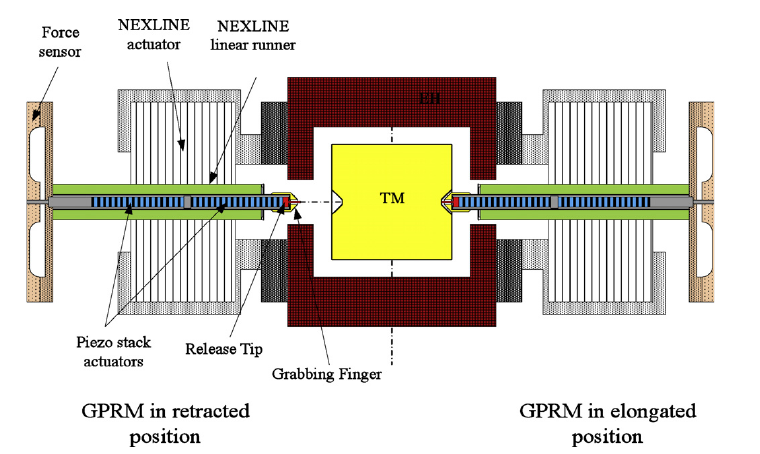
\includegraphics[scale=0.4]{gfx/GPRM}
		\end{centering}
		\caption{GPRM Mechanism}
	\end{figure}
	
	It's main parts are :
	\begin{itemize}
		\item \textit{Grabbing Finger} : holds the TM and positions it prior relase;
		\item \textit{Finger Tip} : last contact part that pons the TM in position before fast retraction for relase;
		\item \textit{Low Voltage Piezo Actuator} : used for the positioning and fast Finger Tip relase;
		\item \textit{NEXLINE actuator} : used for Grabbing Finger movement;
		\item \textit{Displacemente Sensor} : to measure the axial force acting between the mechanism contacting interface;
	\end{itemize}

	\subsubsection{Main Task}
	The model of the injection procedure consist of three parts.\\
	The GPRM, the adhesion phenomenon and the TM motion equations.
	Two opposite GPRMs are operated simultaneously in order to hold the
	TM with the Grabbing Fingers in the center of the Electrode Housing
	(EH). From this configuration, the procedure can be considered to be symmetrical, as the two mechanism are commanded in the same way :	
	\begin{itemize}
		\item \textbf{Pre-launch and launch phase}
		\begin{enumerate}
			\item The TM is held by the Caging Mechanism (CM) at the eight corners;
		\end{enumerate}
		\item \textbf{TM Relase from CM}
		\begin{enumerate}
			\item The Grabbing Finger is in contact with the TM and the tip is fully retracted;
		\end{enumerate}
	\end{itemize}	
	The contact between the GF and the TM has to perform the following
	functions :	
	\begin{description}
		\item [{-}] Fix the TM during the release of the CM;
		\item [{-}] Center the TM in the EH;
		\item [{-}] Orient the TM with respect to the EH;
	\end{description}	
	This contact however not suitable for an undisturbated release for geodesic injection.\\ 
	The release tip must thus take over the TM pinning before
	release. 	
	\begin{itemize}
		\item \textbf{Pass Over}
		\begin{enumerate}
			\item The RT moves forward until a contact force is recorded 
			\item The GF is	retracted a small amount to compensate for the movement of the RT;
			\item The force is then reduced to the lowest acceptable level that still controls the position of the TM;
			\item TM release is performed by means of a fast contraction of the linear piezo actuator, which also commands the retraction of the tips;
			\item The TM is capture by the drag-free attitude and control system and take finally to the 					nominal center of its housing;
		\end{enumerate}
	\end{itemize}	
	We must pay attention to the fact that in presence of adhesion the
	fast retraction may cause a momentum transfer from the RTs to the TM. 

\subsubsection{The Physical System}
    The GPRM can be physically modeled as the lumped-element diagram reported in Figure 2 :  
    
    	\begin{figure}[H]
		\begin{centering}
			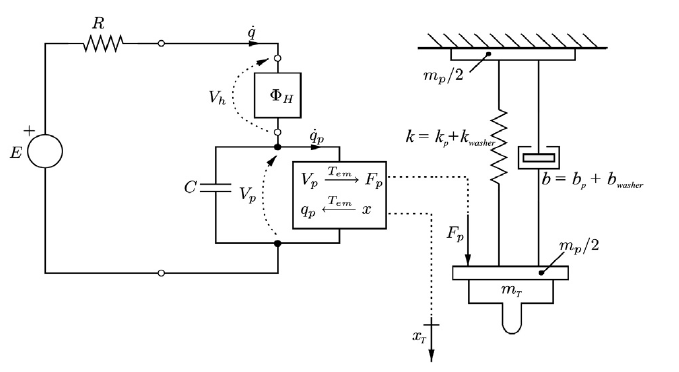
\includegraphics[scale=0.4]{gfx/phys_model}
		\end{centering}
		\caption{GPRM Physical Model}
	\end{figure}
	
	The diagram comprises the release tip mass and washer springs mounted at the extremity of the Grabbing Finger (GF) unit, and the piezo-stack actuator connected to a voltage generator through a discharge resistor R.
	
\subsubsection{The Mathematical Model}
    A mathematical model for the lumped-element freshly shown can be easily derived by resorting to elementary physical laws, such as the Kirchoff laws and Newton's laws, once the constitutive equations of the piezo-stack actuator are known.
    The most conventional model of a piezo-stack actuator is the one which relies on the linear constitutive equations of piezoelectric materials. \todo[inline]{inserire citazione paper} 
    Such model however is not useful for describing the dynamics of piezo-actuated positioning mechanisms because it neglects the intrinsic dynamics of the actuator. 
    A lumped parameter linear model for the piezo actuator can be obtained by manipulating the equations provided in \todo[inline]{inserire citazione paper isteresi} and by neglecting the hysteresis \todo[inline]{inserire citazione paper bortoluzzi 1} .\\
    Using the Newton and Kirchoff's laws, together with the constitutive equations of the piezoelectric transducer, and by neglecting the degree of freedom describing the suspended mass of the piezo stack\todo[inline]{inserire citazione paper bortoluzzi 2} we can obtain the equations governing the simplified model of Fig. 2 :
    \begin{equation}
        RC_{a}\dot{q}(t)+q(t)-T_{em}x_{T}(t)=C_{a}E(t)
    \end{equation}
    
    \begin{equation}
        m\ddot{x}_{T}(t)+ b\dot{x}_{T}(t) + \left(k+\frac{T_{em}^{2}}{C_{a}}\right) x_{T}(t) - \frac{T_{em}}{C_{a}}q(t) = 0
    \end{equation}
    where :
	\begin{itemize}
		\item $E(t)$ is the input voltage
		\item $q(t)$ is the charge accumulated on the piezo
		\item $x_{T}(t)$ is the RT position
		\item $C_{a}$ is the capacitance of the piezo stack
		\item $T_{em}$ is the piezo effect
		\item $m$ is the mass of the RT plus half of the mass of the piezo-stack
		\item $b$ is the damping coefficient
		\item $k$ is the stiffness coefficient
	\end{itemize}
    If the voltage $E$ and the test mass displacement $x_{T}$ are taken as the input and output variables of the system, then we can write the transfer function describing the dynamics of the GPRM as :
    \todo[inline]{ricavare fdt sistema semplificato}
    The system may be written in state space form
    \todo[inline]{copiare equazioni agli stati}    
    
\section{Simulation}
\subsection{Identification}

    \listoftodos
\end{document}
